\documentclass{article}
\usepackage{graphicx} % Required for inserting images
\usepackage[T1]{fontenc}
\usepackage{tgbonum}
\fontfamily{qcr}\selectfont

\usepackage{layout}
\title{\textbf{Project : Stock Insights \& Predictive Analytics Using Machine
Learning}}
\author{\normalsize Krish Singhvi(PID:730542655), Nandan Mogili(PID:730573354), Soham Joshi(PID:730559240)}
\date{UNC Chapel Hill, December 2024}
\usepackage{blindtext}
\usepackage{geometry}
 \geometry{
 a4paper,
 total={170mm,257mm},
 left=20mm,
 top=20mm,
 }
\begin{document}
\maketitle


\textbf{\Large Abstract}
\newline
The stock market is a complex, volatile environment influenced by a myriad of factors, making accurate prediction a significant challenge. This project leverages Long Short-Term Memory (LSTM) networks, a deep learning technique, to develop a robust predictive model for stock price forecasting. By integrating real-world data from Yahoo Finance API, pre-processing it with Python libraries like Pandas and Scikit-learn, and visualizing insights using Matplotlib, the model captures temporal dependencies in financial data effectively. This work provides valuable insights into building scalable, accurate prediction models, aiding in investment decisions.



\section{Introduction}
Stock price prediction, a critical component of financial forecasting, is inherently difficult due to the dynamic nature of market conditions. Traditional methods often fail to capture the nonlinear patterns present in financial data. In this project, we address this limitation by employing Long Short-Term Memory (LSTM) networks, which excel in analyzing sequential data and uncovering long-term dependencies.
\newline \newline 
The objective of this project is to develop a predictive pipeline that processes real-world financial data, builds an accurate forecasting model, and visualizes actionable insights. By combining real-time data integration, advanced pre-processing techniques, and deep learning models, this project provides a scalable solution for stock market forecasting.


\section{Methodology}
\vspace{10pt}
\setlength{\marginparwidth}{0pt}
\setlength{\marginparsep}{0pt}
\subsection{Data Collection}

The dataset used in this project was obtained through the Yahoo Finance Market Data API, which provides real-time and historical stock market data. Key features include:

\begin{itemize}
\item {{\textbf{Open, High, Low, Close Prices: }}}Essential for understanding daily price movements.The default journal template style.
\item {\textbf{{Volume: }}}A measure of market activity and investor interest.
\item {{\textbf{Adjusted Close Prices: }}}Reflect dividends, stock splits, and other adjustments.
\end{itemize}
For this project we used Apple Inc Stock (Ticker – AAPL). A fourteen-year dataset was collected for analysis to ensure sufficient training data and long-term trend analysis.

Open and Close price of Apple Stock (AAPL) over time based on data collected using Yahoo Finance API leveraging Pandas Data Frame and Matplotlib. This helps in understanding the trends and relationships between the opening and closing prices of the stock.
\newline 
\newline 

\begin{figure}[h]
  \centering
  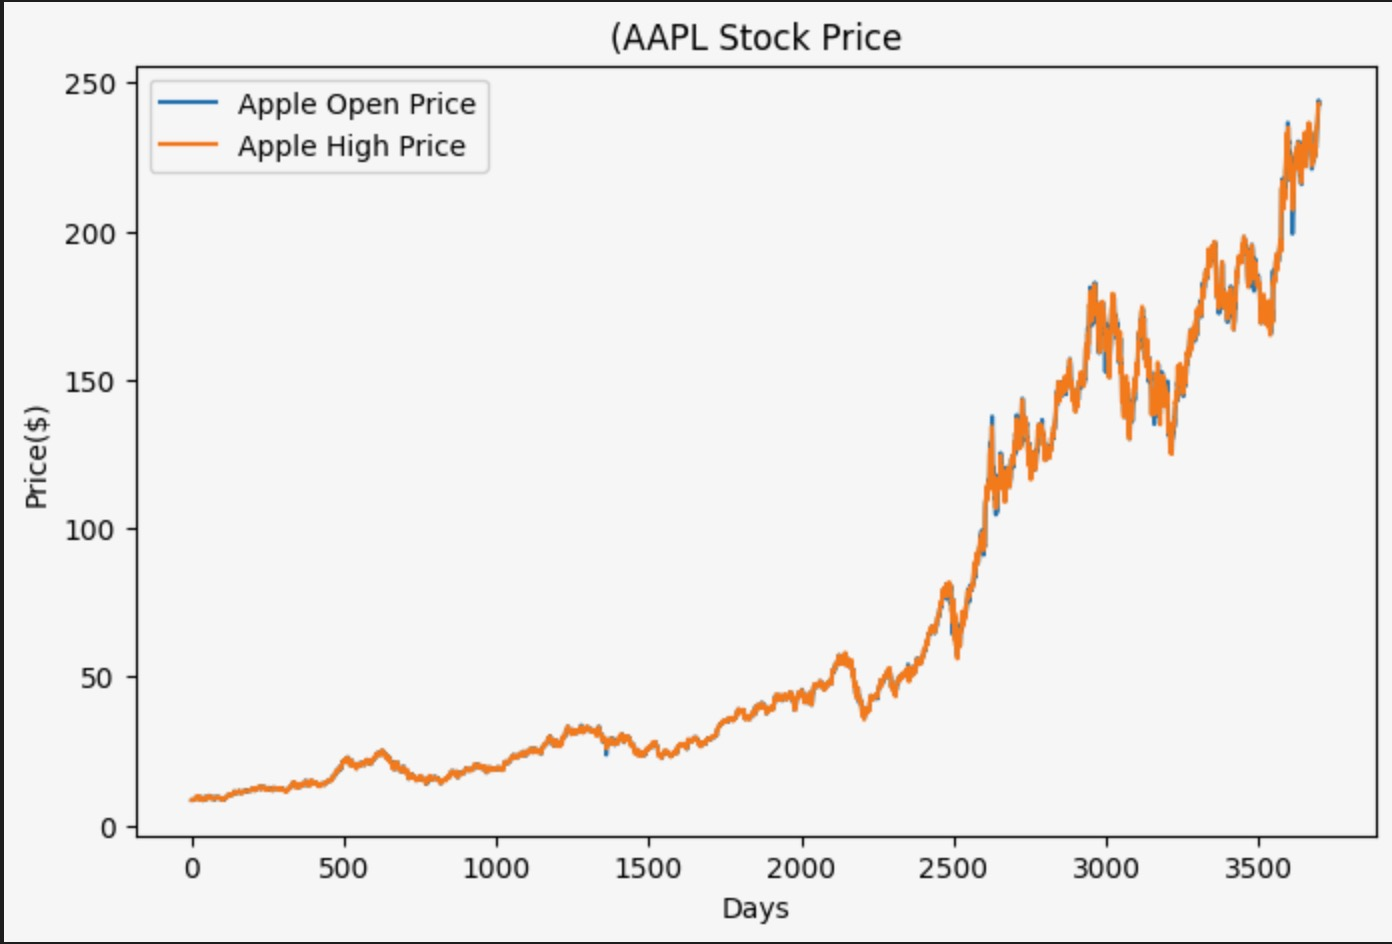
\includegraphics[width=\linewidth]{APPL Open Close.png}
  \caption{ Open and Close price of Apple Stock (AAPL)}
  \Description{}
\end{figure}

\subsection{Data Preprocessing}

Data preprocessing is critical for ensuring model performance and accuracy. The following steps were implemented:

\begin{itemize}
\item {{\textbf{Handling Missing Data:  }}Missing values were addressed using forward-fill methods, ensuring data continuity for time-series analysis.
\item {{\textbf{Feature Scaling:}}MinMaxScaler from Scikit-learn’s module was applied to normalize features between 0 and 1, reducing the impact of scale differences on model training . LSTMs, like many machine learning algorithms, require input data to be normalized to ensure effective learning. This scaler maps data to a specified range, typically between 0 and 1.
\item {{\textbf{Train-Test Split:  }}The dataset (stock price data) was divided into 80\% for training and 20\% for testing, ensuring the model generalizes well to unseen data. This section prepares the data for training and testing a supervised machine learning model, such as LSTM, by splitting the stock price data into training and testing datasets.
\item {{\textbf{Handling Missing Data:  }}Missing values were addressed using forward-fill methods, ensuring data continuity for time-series analysis.
\item {{\textbf{Data Conversion : }}Convert Input data to in numerical array required by LSTM models for compatibility with TensorFlow/Keras libraries.
\newline 
\newline 
\newline
\newline 
\newline 
\newline 
\newline 
\newline 
\newline 
\end{itemize}

\begin{figure}[h]
  \centering
  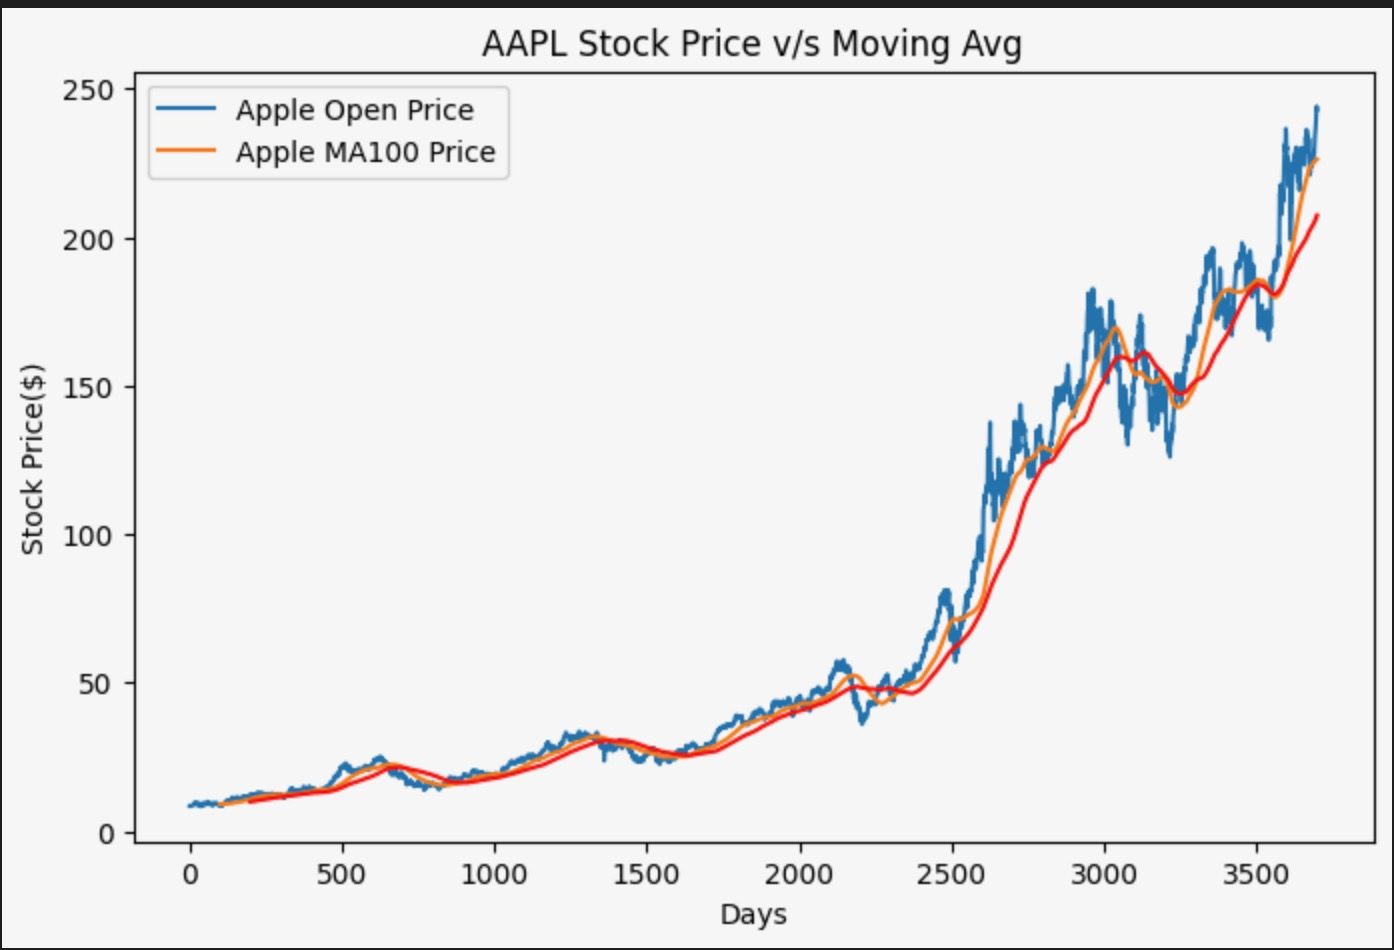
\includegraphics[width=\linewidth]{APPL MOV Avg.png}
  \caption{ Calculate Moving Average 100 and 200 Days of Apple Stock (AAPL)}
  \Description{}
\end{figure}

\subsection{Model Architecture}

The predictive model was built using Keras with TensorFlow as the backend. The architecture was designed to balance complexity and performance and is well-suited for time-series data, like stock prices, as it can retain information over long sequences.
\begin{itemize}
\item {{\textbf{LSTM Layer:}}A mutiple LSTM layer with 50 units to capture sequential patterns in the data. To balances model complexity and computational efficiency. Adding multiple LSTM layers helps the model capture hierarchical patterns in the data. 
\item {{\textbf{Dropout Layer: }}Introduced a dropout rate of 0.2 to prevent over-fitting.
\item {{\textbf{Dense Output Layer: }} single neuron to output the predicted stock price. The Dense layer is the final layer of the network, used to generate final output for stock price prediction.
\item {{\textbf{Adam optimizer : }}The Adam optimizer was used for training with a learning rate of 0.001. Adam is widely used because it is computationally efficient, handles sparse gradients well.
\item {{\textbf{Mean Squared Error :}}The loss function was set to Mean Squared Error (MSE), for regression tasks. MSEis suitable for time-series forecasting tasks like stock price prediction, where accurate predictions are critical.
\item {{\textbf{Epochs :} }Our Model used 50 epochs, which is a reasonable starting value to balance computational efficiency and performance.
\end{itemize}

\section{Results and Discussion}

Below Figure presents a comparison of predicted versus actual stock prices of Apple Inc Stock, illustrating the model's accuracy in following market trends. The visualization highlights the model’s capability to capture both short-term fluctuations and long-term trends.
\begin{figure}[h]
  \centering
  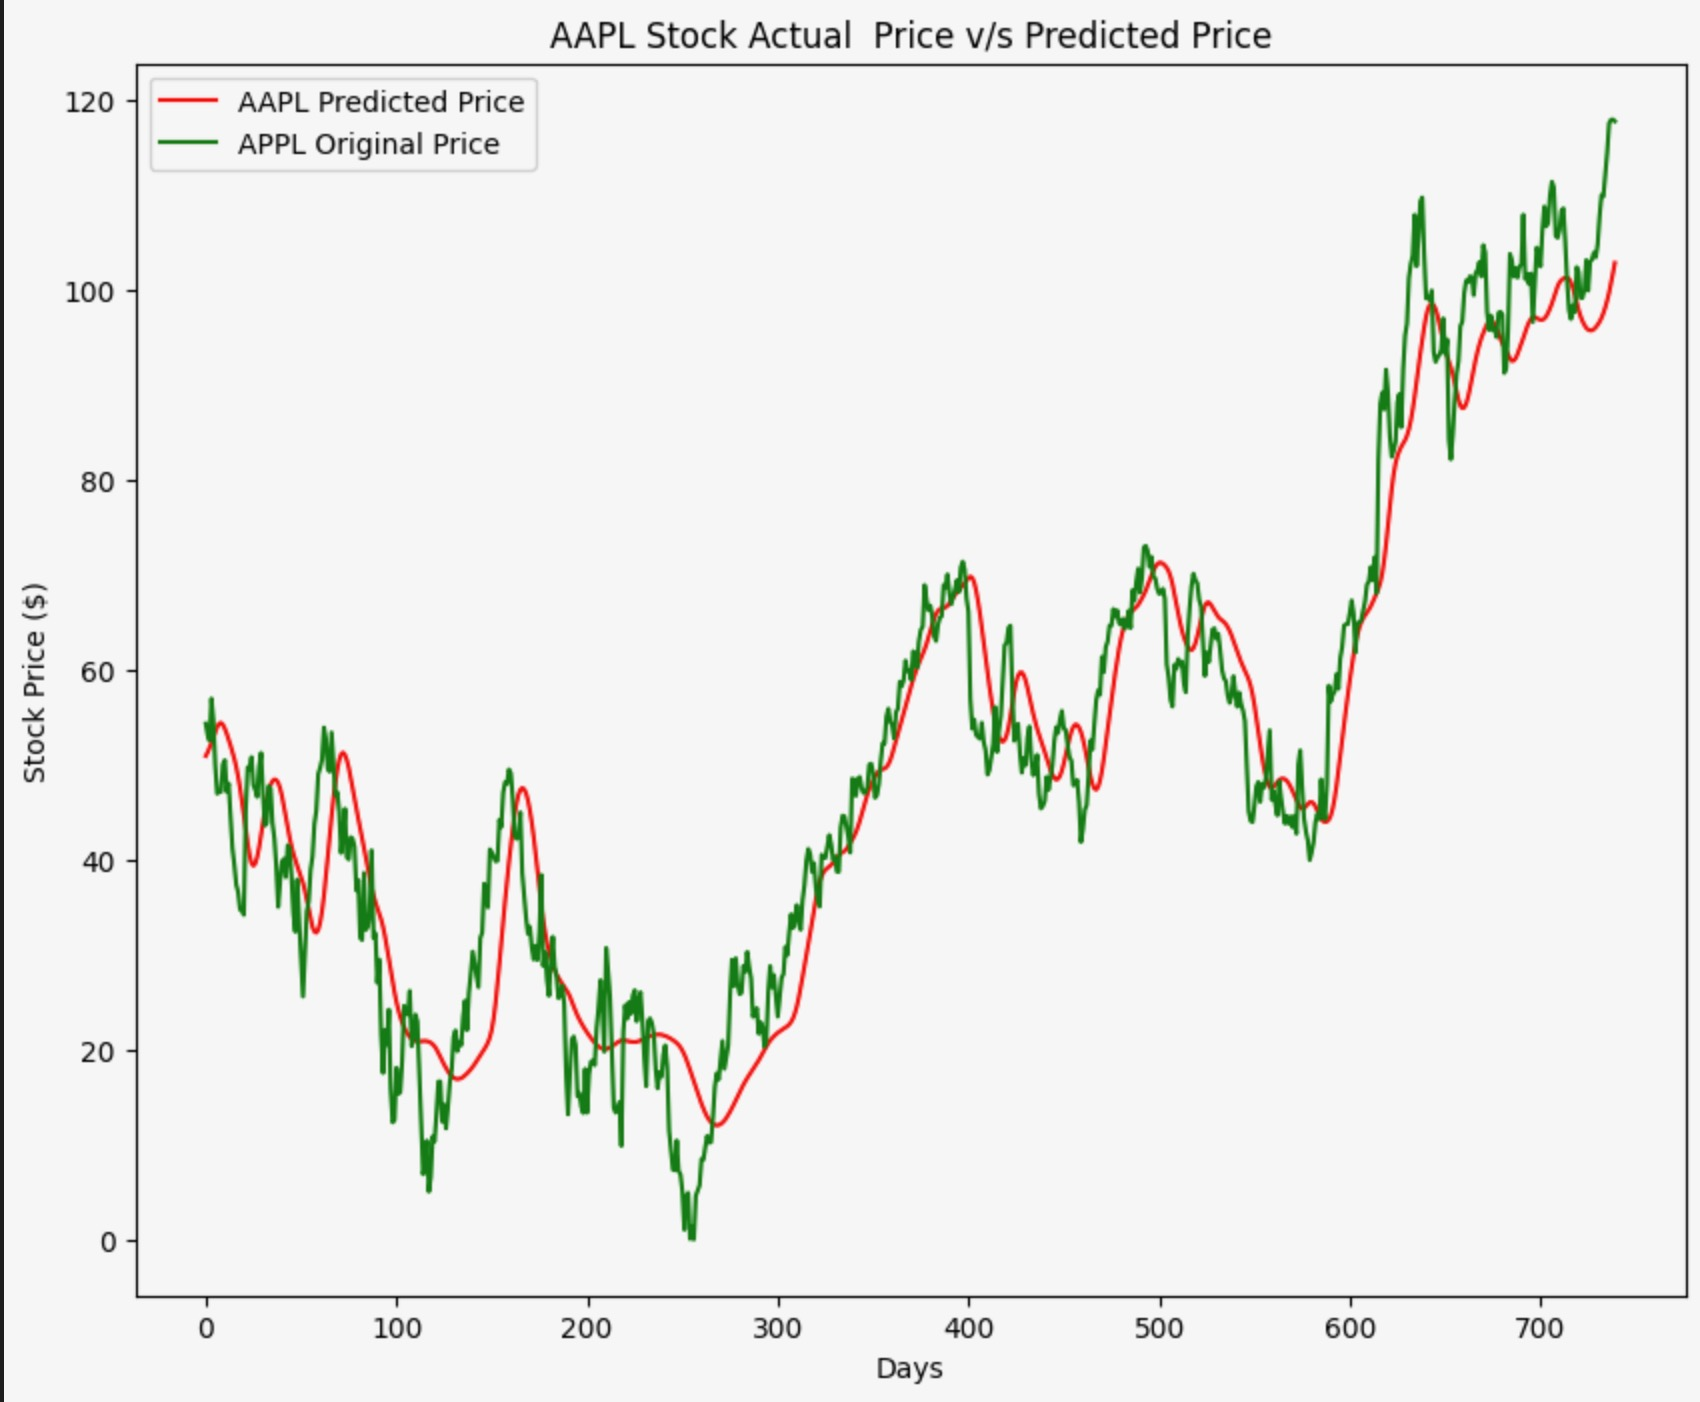
\includegraphics[width=\linewidth]{Appl Actual to Predict.png}
  \caption{ Actual v/s Predicted Price of Apple Stock (AAPL) based on Machine Learning Project}
  \Description{}
\end{figure}



\begin{itemize}
\item {{\textbf{Effectiveness of LSTM: }}The model effectively captures sequential patterns in financial data (Apple Inc Stock Price), outperforming traditional methods.
\item {{\textbf{Impact of Pre-processing: }}Proper feature scaling and data cleaning significantly improved model performance.
%\item {{\textbf{Scalability:  }}The methodology is adaptable to other financial datasets and markets, making it a versatile tool for investors.
\end{itemize}


\section{Conclusions and Future Work}

\subsection{ Conclusions}
This project demonstrates the potential of deep learning, particularly LSTM networks, in financial forecasting as shown for Apple Inc Stock Price. By integrating real-time data and applying advanced pre-processing techniques, the project achieved a reliable predictive model with high accuracy.
%The methodology is scalable and applicable to various financial scenarios, providing a valuable tool for investment decision-making.

\subsection{ Future Directions}


\begin{itemize}
\item {{\textbf{Incorporating Additional Features: }}Future work could include macroeconomic indicators and news sentiment analysis to enhance prediction accuracy.
%\item {{\textbf{Exploring Ensemble Models:  }}Combining LSTM with other machine learning techniques could further improve performance.
\item {{\textbf{Real-Time Prediction Pipelines with User Interface: }}Developing a pipeline for live data streaming and prediction with User Interface would extend the model's practical applications.
\end{itemize}

\section{Acknowledgments}

We would like to thank Prof. Jorge Silva for his invaluable guidance and support throughout the course of COMP 562.

\section{References}

[1].	Hochreiter, S., \& Schmidhuber, J. (1997). Long Short-Term Memory. Neural Computation. 
\newline
\newline
[2].	Kim, K., \& Han, I. (2000). Genetic algorithms approach to feature discretization in artificial neural networks for prediction of stock price index.
\newline
\newline
[3].Emerson, S., Kennedy, R., O’Shea, L., & O’Brien, J. (2019, May). Trends and Applications of Machine Learning in Quantitative Finance
\newline
\newline
[4] Heaton J.B., Polson N.G., Witte J.H. Deep learning for finance: deep portfolio
\newline
\newline
[5] FischerThomas et al. (2018)
Deep learning with long short-term memory networks for financial market predictions
\newline
\newline
[6] Ahmet Murat Ozbayoglu Omer Berat Sezer, in 
Applied Soft Computing
, (2020) Deep learning for financial applications : A survey
 \section{GitHub Repository}
The complete codebase and detailed documentation for this project are available at:
\newline
\newline
\url{https://github.com/krishsinghvi/COMP562}.

\end{document}
endinput
%%
%% End of file `sample-acmsmall.tex'.


\end{document}
